\documentclass[serif,mathserif]{beamer}

\usepackage{sqrcaps}
\usepackage[T1]{fontenc}

\usepackage{amsmath, amssymb, amsfonts, epsfig, xspace}
\usepackage{mathtools}
\usepackage{pstricks,pst-node}
\usepackage{multimedia}
\usepackage[normal,tight,center]{subfigure}
\setlength{\subfigcapskip}{-.5em}
\usepackage{beamerthemesplit}
\usetheme{lankton-keynote}

\newcommand{\AAA}{\mathfrak A}
\newcommand{\DDD}{\mathfrak D}
\newcommand{\BBB}{\mathcal B}
\newcommand{\CCC}{\mathcal C}
\newcommand{\HHH}{\mathcal H} %for Hilbert space
\newcommand{\LLL}{\mathcal L} % for lattice
\newcommand{\MMM}{\mathcal M}

\newcommand{\Lat}{\mathcal Lat}
\newcommand{\Alg}{\mathcal Alg}
\newcommand{\tr}{\tau}
\newcommand{\C}{\mathbb C} %for complex number
\newcommand{\R}{\mathbb R}  %for real number
\newcommand{\Z}{\mathbb Z} %for integer
\newcommand{\N}{\mathbb N} % for nature number
\newcommand{\T}{\mathbb T} % tours
\newcommand{\acts}{\curvearrowright}

\author[W. Yuan \& W. Wu]{Wenming Wu(CQNU) \quad Wei Yuan(AMSS)}

\title[\hspace{2em}\insertframenumber/\inserttotalframenumber]
{Unbounded Operator With Trivial Relative Commutant}

\date[]{Nov.2 2013} %leave out for today's date to be insterted

\institute{Dartmouth College}

\begin{document}

\maketitle

\section{Preliminary}  % add these to see outline in slides

\begin{frame}
\frametitle{Notations}
\begin{itemize}
  \item $\AAA$: finite von Neumann algebra \pause
  \item An unbounded operator $T$ with domain $\DDD(T)$ is said to be
        closed if its graph $G(T) = \{(\xi, T\xi): \xi \in \DDD(T)\}$ is
        closed. \pause
  \item A \textbf{closed densely defined} operator $T$ is \textbf{affliated} with
    a von Neumann algebra $\AAA$, and write $T \eta \AAA$, when
    $$U^{*}TU = T$$ 
    for each unitary $U$ in $\AAA'$. \pause
    $$U \DDD(T) = \DDD(T)$$
\end{itemize}
\end{frame}


\begin{frame}
    \begin{figure}[t]
    \centering
      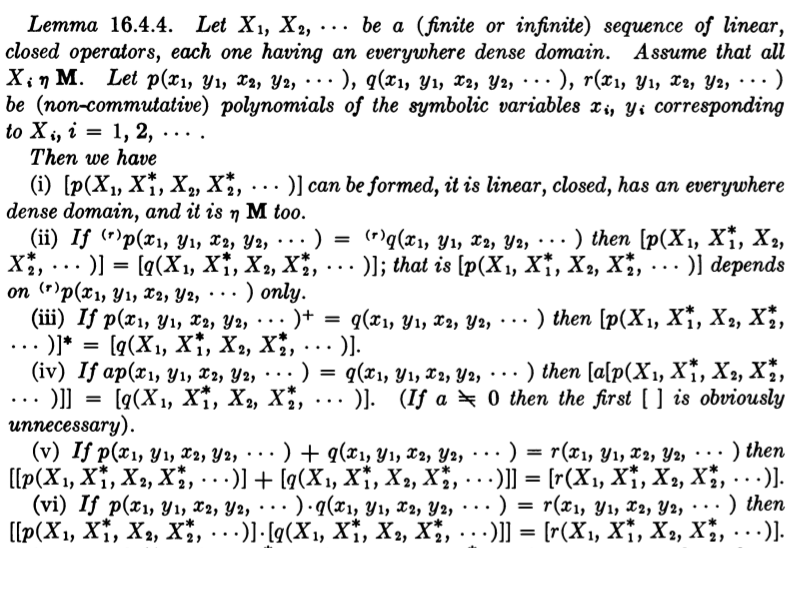
\includegraphics[scale=0.3]{vm.png}
      \caption{\small{On Rings of Operators(1936)}}
  \end{figure}
\end{frame}


\begin{frame}
  \frametitle{Questions}
   The family of operators affiliated with a finite von Neumann algebra
   is a * algebra (with unit $I$). &
  \begin{itemize}
      \visible<2>{\item Is there a $T \eta \AAA$ such that 
          $T' \cap \AAA = \{\C I\}$?} &
      \visible<3>{\item Is there a $T \eta \AAA$ such that $T$ does not 
          commute with any non trivial normal operator in $\AAA$?}
  \end{itemize}
\end{frame}

\section{Fuglede-Putnam Theorem}

\begin{frame}
  \frametitle{Fuglede-Putnam Theorem}
  If $T$ is a bounded operator and if $M$ and $N$ are (closed) normal operators, then
  \pause
   $$TN \subset MT$$  \pause 
   $$\Rightarrow TN^{*} \subset M^{*}T$$
\end{frame}

\begin{frame}
\begin{lemma}
   Let $\AAA$ be a finite von Neumann algebra. 
   If $N$ is a normal operator and $P$ is a projection such that 
   $(I-P)NP = 0$, then $PN = NP$.
\end{lemma}
\end{frame}

\begin{frame}
\begin{lemma}
    Let $\AAA$ be a finite von Neumann algebra,
    and $H$ is a closed positive operator affiliated with $\AAA$. 
    If $M$ and $N$ are normal operators in $\AAA$ and $NH = HM$, then
    $NH=HN$, $MH = HM$ and $M^{*}H = HN^{*}$.
\end{lemma}
\end{frame}
%\section{Conclusion} % add these to see outline in slides

\begin{frame}
\begin{proof}
\renewcommand{\qedsymbol}{} % do not show square at the end!
    \only<1>{We assume that $Ker(H) = \{0\}$ and 
    $$H = \int_{0}^{\infty} \lambda d E_{\lambda}$$} &
    \only<2>{
    $$P = E_{\lambda} = \begin{pmatrix}
          I & 0\\
          0 & 0
      \end{pmatrix} \quad 
   H = \begin{pmatrix}
       H_1 & 0\\
       0 & H_2
   \end{pmatrix} $$  
   $$N = \begin{pmatrix}
       N_{11} & N_{12}\\ 
       N_{21} & N_{22} \\
   \end{pmatrix}, \quad  
   M = \begin{pmatrix}
       M_{11} & M_{12}\\ 
       M_{21} & M_{22} \\
   \end{pmatrix} $$} &
   \only<2->{$H_1 = HE_{\lambda}$, $\| H_{1} \| \leq \lambda$ and 
   $H_2 = H(I-E_{\lambda})$, $\|H_{2}^{-1}\| \leq \frac{1}{\lambda}$}
   \only<3-5>{$$NH = HM$$} 
   \only<4-5>{$$\Rightarrow
    \begin{pmatrix}
        H_{1}^{-1}N_{11}H_{1} & H_{1}^{-1}N_{12}H_{2}\\
        H_{2}^{-1}N_{21}H_{1} & H_{2}^{-1}N_{22}H_{2}\\
    \end{pmatrix} = 
    \begin{pmatrix}
        M_{11} & M_{12}\\ 
        M_{21} & M_{22} \\
    \end{pmatrix}$$}
    \only<5>{
        $$ \Rightarrow \tau|_{P\AAA P}(H_{1}N_{21}^{*}H_{2}^{-2}N_{21}H_{1}) 
        = \tau|_{P\AAA P}(H_{1}^{-1}N_{12}H_{2}^{2}N_{12}^{*}H_{1}^{-1})$$ 
    }
    \begin{align*}
        \only<6-9>{\tau \left (
        \begin{pmatrix}
            H_{1}N_{21}^{*}H_{2}^{-2}N_{21}H_{1} & 0\\
            0 & 0
        \end{pmatrix} \right)
        &\leq  \frac{1}{\lambda^{2}}
        \tau \left (
        \begin{pmatrix}
            H_{1}N_{21}^{*}N_{21}H_{1} & 0 \\
            0 & 0
    \end{pmatrix} \right) \\}
    & \only<7-9>{ = \frac{1}{\lambda^{2}} \tau \left (
         \begin{pmatrix}
             0 & H_1 N_{21}^{*}\\
             0 & 0
         \end{pmatrix}
         \begin{pmatrix}
             0 & 0\\
             N_{21}H_1 & 0
         \end{pmatrix}
     \right )\\} 
     & \only<8->{ = \frac{1}{\lambda^{2}} \tau \left (
        \begin{pmatrix}
            0 & 0\\
            0 & N_{21}H_{1}^{2}N_{21}^{*}
         \end{pmatrix}
     \right ) \\}
     & \only<9>{\leq \tau \left (
        \begin{pmatrix}
            N_{21}^{*}N_{21} & 0\\
            0 & 0 
         \end{pmatrix}
     \right )}
    \end{align*}
    
\end{proof} 
\end{frame}

\begin{frame}
    \begin{proof}
\renewcommand{\qedsymbol}{} % do not show square at the end!
        \only<1-4>{
         $$ \tau \left (
        \begin{pmatrix}
            H_{1}N_{21}^{*}H_{2}^{-2}N_{21}H_{1} & 0\\
            0 & 0
        \end{pmatrix} \right)
         \leq \tau \left (
        \begin{pmatrix}
            N_{21}^{*}N_{21} & 0\\
            0 & 0 
         \end{pmatrix}
     \right ) $$
    }
    \only<2-4>{Let $Q = E_{\beta} - E_{\lambda}$, $\beta > \lambda$
    \begin{align*}
        \frac{\beta^{2}}{\lambda^2}\tau \left (
    \begin{pmatrix}
        N_{12}(I-Q)N_{12}^{*} & 0\\
        0 & 0
    \end{pmatrix} \right )
     & + \tau \left (
    \begin{pmatrix}
        N_{12}QN_{12}^{*} & 0\\
        0 & 
    \end{pmatrix} \right ) \\ 
    & \leq
    \tau \left (
    \begin{pmatrix}
        H_{1}^{-1}N_{12}H_{2}^{2}N_{12}^{*}H^{-1} & 0\\
        0 & 0
    \end{pmatrix} \right) 
    \end{align*}
    }
    \only<3>{
      \begin{align*}
    \tau \left(
    \begin{pmatrix} 
        N_{12}N_{12}^{*} & 0 \\
        0 & 0 \\
    \end{pmatrix}
    \right )= 
    \tau \left (
    \begin{pmatrix} 
        N_{21}^{*}N_{21} & 0 \\
        0 & 0
    \end{pmatrix}    
    \right )
\end{align*}
    }
    \only<4>{
    \begin{align*}
        \frac{\beta^{2}}{\lambda^2}\tau \left (
        \begin{pmatrix}
            N_{12}(I-Q)N_{12}^{*} & 0\\
            0 & 0
        \end{pmatrix} \right ) \leq
        \tau \left(
        \begin{pmatrix} 
            N_{12}(I-Q)N_{12}^{*} & 0 \\
            0 & 0 \\
    \end{pmatrix}
        \right )
    \end{align*}
    } 
    \end{proof}
\end{frame}

\begin{frame}
   \begin{proof}
\renewcommand{\qedsymbol}{} % do not show square at the end!
     \begin{align*}
         \only<1-> {\frac{\beta^{2}}{\lambda^2}\tau \left (
        \begin{pmatrix}
            N_{12}(I-Q)N_{12}^{*} & 0\\
            0 & 0
        \end{pmatrix} \right ) &\leq
        \tau \left(
        \begin{pmatrix} 
            N_{12}(I-Q)N_{12}^{*} & 0 \\
            0 & 0 \\
    \end{pmatrix}
\right )} \\
& \only<2-> {\Downarrow \\}
\only<3->{ N_{12}N^{*}_{12} &= 0 \\}
\only<4>{& \Downarrow \\}
    \end{align*}
   \end{proof} 
\end{frame}

\begin{frame}
    \begin{proof}
     \begin{align*}
         \frac{\beta^{2}}{\lambda^2}\tau \left (
        \begin{pmatrix}
            N_{12}(I-Q)N_{12}^{*} & 0\\
            0 & 0
        \end{pmatrix} \right ) &\leq
        \tau \left(
        \begin{pmatrix} 
            N_{12}(I-Q)N_{12}^{*} & 0 \\
            0 & 0 \\
    \end{pmatrix}
\right ) \\
& \Downarrow \\
 N_{12}N^{*}_{12} &= 0 \\
                            & \Downarrow \\
E_{\lambda}N = NE_{\lambda} & \mbox{ and } NH = HN
    \end{align*}
\end{proof} 

\end{frame}

\begin{frame}
    \only<1->{\begin{theorem}
    Let $\AAA$ be a finite von Neumann algebra,
    and $T$ a closed operator affiliated with $\AAA$. 
    If $N$ is a normal operator in $\AAA$ and $NT = TN$, then
    $N^{*}T = TN^{*}$.
\end{theorem}}

\only<2>{\begin{corollary}
    Let $\AAA$ be a finite von Neumann algebra,
    and $T$ is a closed operator affiliated with $\AAA$. 
    If $N$ and $M$ are normal operators affiliated with 
    $\AAA$ and $MT = TN$, then $M^{*}T = TN^{*}$.
\end{corollary}}

\only<3>{\begin{corollary}
   If $\AAA$ be a separable II$_1$ factor, then there exists 
   a closed operator $T$ affiliated with $\AAA$ such that 
   $NT \neq NT$ for any nontrivial normal operator affiliated with 
   $\AAA$.
\end{corollary}}
\end{frame}

\begin{frame}
    \begin{center}
        Is there a $T \eta \AAA$ such that $T' \cap \AAA = \{\C I\}$?
    \end{center}
\end{frame}

\section{A Humble Example}

\begin{frame}
\begin{center}
    $\Z  \acts (\T, \mu): \alpha(n)e^{2\pi i\theta} = 
e^{2\pi i(n\alpha + \theta)}  \mbox{ $\alpha$ is irrational}$
\end{center} \pause

\begin{itemize}
    \item measure preserving \pause
    \item ergodic, i.e. $X \subset \T$ and $\mu(\alpha(n)(X) \setminus X) = 0$ \\
         $\Rightarrow \mu(X) = 0$ or $\mu(\T \setminus X) = 0$. \pause
\end{itemize}

\begin{center}
   $\Downarrow$\\ \pause
   $L^{\infty}(\T)\rtimes_{\alpha} \Z (\subset 
   \BBB(L^{2}(\T)\otimes l^{2}(\Z))$ is the hyperfinite II$_1$ 
   factor $\mathcal{R}$\\ \pause
   $\sum_{n} \alpha(-n)(h) \otimes E_{n}, \qquad I \otimes l_{n}
   \qquad h \in L^{\infty}(\T)$
\end{center}
\end{frame}

\begin{frame}
   \begin{center}
       $h(\theta) = \frac{e^{2\pi i \theta} + 1}{e^{2\pi i \theta} -1}$ \\ \pause
       \vspace{0.5cm}
       $T = \sum_{n}\alpha(-n)(h) \otimes E_{n}l_{1}$ \\ \pause
        \vspace{0.5cm}
       $T$ is a densely defined closed operator affiliated with $\mathcal{R}$ \\
       \pause
       \vspace{0.5cm}
       $AT \neq TA$ for each $A \in \mathcal{R} \setminus \{\C I\}$       
   \end{center} 
\end{frame}

\begin{frame}
    $$h(\theta) = \frac{e^{2\pi i \theta} + 1}{e^{2\pi i \theta} -1}$$ 
    \only<1->{
    \begin{center}
    $A = \sum_{m} \sum_{n}\alpha(-n)(f_{n}) \otimes E_{n}l_{m}$ \\ 
    \end{center}}
    \begin{align*}
        \only<2->{AT &= TA \\}
        & \only<3->{\Downarrow \\}
        \only<4->{\frac{\alpha(1)(f_{n})}{f_{n}} 
        &= \frac{\alpha(n)(h)}{h}}
    \end{align*}
\end{frame}

\begin{frame}
    \only<1-> {\begin{align*}
   k_{m} =  \begin{cases}
       h\alpha(1)(h)\cdots\alpha(m-1)(h) &\mbox{ if } m > 0 \\
       1 &\mbox{ if } m = 0 \\
       \alpha(-1)(\frac{1}{h})\alpha(-2)(\frac{1}{h})
       \cdots\alpha(m)(\frac{1}{h}) &\mbox{ if } m < 0
   \end{cases} 
\end{align*}}


\begin{align*}
    \only<3->{&\Downarrow \\
    \alpha(\frac{f_{m}}{k_{m}}) &= \frac{f_{m}}{k_{m}} \\}
    \only<4>{ &\Downarrow \\ 
f_{m} &= \lambda k_{m}} 
\end{align*} 
\end{frame}

\begin{frame}
    \begin{center}
        \sqrcfamily{\Huge{Thank You!}} 
    \end{center}
\end{frame}
\end{document}


